\documentclass[tikz,border=4pt]{standalone}
\usepackage[T1]{fontenc}
\usepackage{helvet}\usepackage{courier}
\renewcommand{\familydefault}{\sfdefault}
\usetikzlibrary{arrows.meta,fit,backgrounds,calc}
\begin{document}
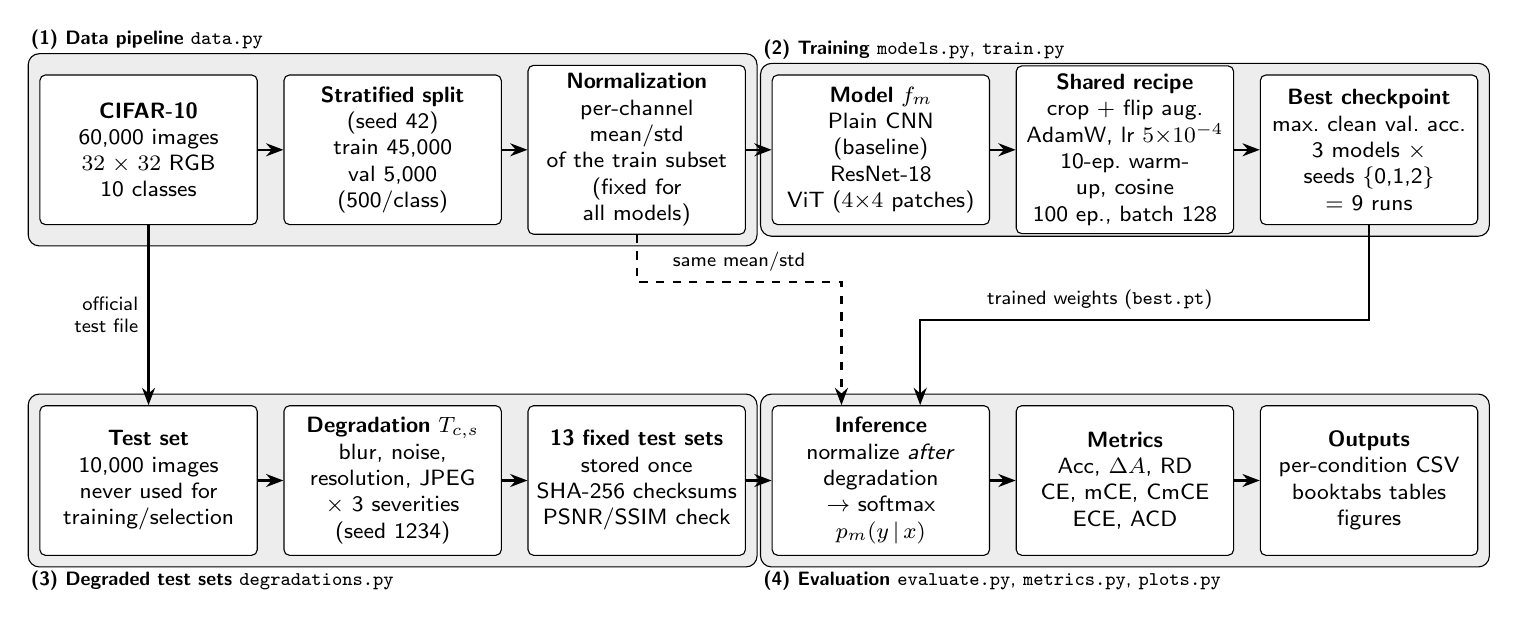
\begin{tikzpicture}[
  font=\footnotesize,
  box/.style={draw, rounded corners=2pt, fill=white, align=center, inner sep=3pt,
              minimum height=19mm, text width=25.5mm},
  arr/.style={-{Stealth[length=2.2mm]}, thick},
  darr/.style={arr, dashed},
  stage/.style={draw, rounded corners=4pt, fill=black!7, inner xsep=4pt, inner ysep=4pt},
  tag/.style={font=\scriptsize\bfseries, anchor=south west, inner sep=1pt}
]
\def\dx{31mm}\def\ry{0}\def\rb{-42mm}
% ---------------- row 1: data + training
\node[box] (cifar)  at (0*\dx,\ry) {\textbf{CIFAR-10}\\60{,}000 images\\$32\times32$ RGB\\10 classes};
\node[box] (split)  at (1*\dx,\ry) {\textbf{Stratified split}\\(seed 42)\\train 45{,}000\\val 5{,}000 (500/class)};
\node[box] (norm)   at (2*\dx,\ry) {\textbf{Normalization}\\per-channel mean/std\\of the train subset\\(fixed for all models)};
\node[box] (model)  at (3*\dx,\ry) {\textbf{Model} $f_m$\\Plain CNN (baseline)\\ResNet-18\\ViT ($4{\times}4$ patches)};
\node[box] (recipe) at (4*\dx,\ry) {\textbf{Shared recipe}\\crop + flip aug.\\AdamW, lr $5{\times}10^{-4}$\\10-ep.\ warm-up, cosine\\100 ep., batch 128};
\node[box] (ckpt)   at (5*\dx,\ry) {\textbf{Best checkpoint}\\max.\ clean val.\ acc.\\3 models $\times$\\seeds \{0,1,2\}\\= 9 runs};
% ---------------- row 2: test sets + evaluation
\node[box] (test)   at (0*\dx,\rb) {\textbf{Test set}\\10{,}000 images\\never used for\\training/selection};
\node[box] (deg)    at (1*\dx,\rb) {\textbf{Degradation} $T_{c,s}$\\blur, noise,\\resolution, JPEG\\$\times$ 3 severities\\(seed 1234)};
\node[box] (sets)   at (2*\dx,\rb) {\textbf{13 fixed test sets}\\stored once\\SHA-256 checksums\\PSNR/SSIM check};
\node[box] (infer)  at (3*\dx,\rb) {\textbf{Inference}\\normalize \emph{after}\\degradation\\$\to$ softmax\\$p_m(y\,|\,x)$};
\node[box] (metr)   at (4*\dx,\rb) {\textbf{Metrics}\\Acc, $\Delta A$, RD\\CE, mCE, CmCE\\ECE, ACD};
\node[box] (out)    at (5*\dx,\rb) {\textbf{Outputs}\\per-condition CSV\\booktabs tables\\figures};
% ---------------- arrows
\draw[arr] (cifar) -- (split);
\draw[arr] (split) -- (norm);
\draw[arr] (norm) -- (model);
\draw[arr] (model) -- (recipe);
\draw[arr] (recipe) -- (ckpt);
\draw[arr] (cifar) -- node[left, font=\scriptsize, align=right]{official\\test file} (test);
\draw[arr] (test) -- (deg);
\draw[arr] (deg) -- (sets);
\draw[arr] (sets) -- (infer);
\draw[arr] (infer) -- (metr);
\draw[arr] (metr) -- (out);
\draw[arr] (ckpt.south) -- ++(0,-12mm) -| node[pos=0.3, above, font=\scriptsize]{trained weights (\texttt{best.pt})} ([xshift=5mm]infer.north);
\draw[darr] (norm.south) -- ++(0,-6mm) -| node[pos=0.25, above, font=\scriptsize]{same mean/std} ([xshift=-5mm]infer.north);
% ---------------- stage frames
\begin{scope}[on background layer]
\node[stage, fit=(cifar)(norm)] (s1) {};
\node[stage, fit=(model)(ckpt)] (s2) {};
\node[stage, fit=(test)(sets)] (s3) {};
\node[stage, fit=(infer)(out)] (s4) {};
\end{scope}
\node[tag] at (s1.north west) {(1) Data pipeline \textmd{\texttt{data.py}}};
\node[tag] at (s2.north west) {(2) Training \textmd{\texttt{models.py}, \texttt{train.py}}};
\node[tag, anchor=north west] at (s3.south west) {(3) Degraded test sets \textmd{\texttt{degradations.py}}};
\node[tag, anchor=north west] at (s4.south west) {(4) Evaluation \textmd{\texttt{evaluate.py}, \texttt{metrics.py}, \texttt{plots.py}}};
\end{tikzpicture}
\end{document}
